%POLAR COORDINATES
%The print template for A4 paper (portrait)
%Author: Zoran Nikolic
\documentclass[12pt]{article}
\usepackage[margin=0.5in,paper=a4paper]{geometry} %Shrinking margins to 0.5in
\usepackage[x11names]{xcolor}                     %Additional colors
\usepackage{tikz}
\usepackage{euler}                                %Nicer numbers

%Note about the colors: 
%  The color of the "ray" lines should not be
%  black or gray as on some printers, significant
%  aliasing distorsion becomes visible.

\begin{document}
\thispagestyle{empty} %Please, no page numbers or similar

\begin{center}
  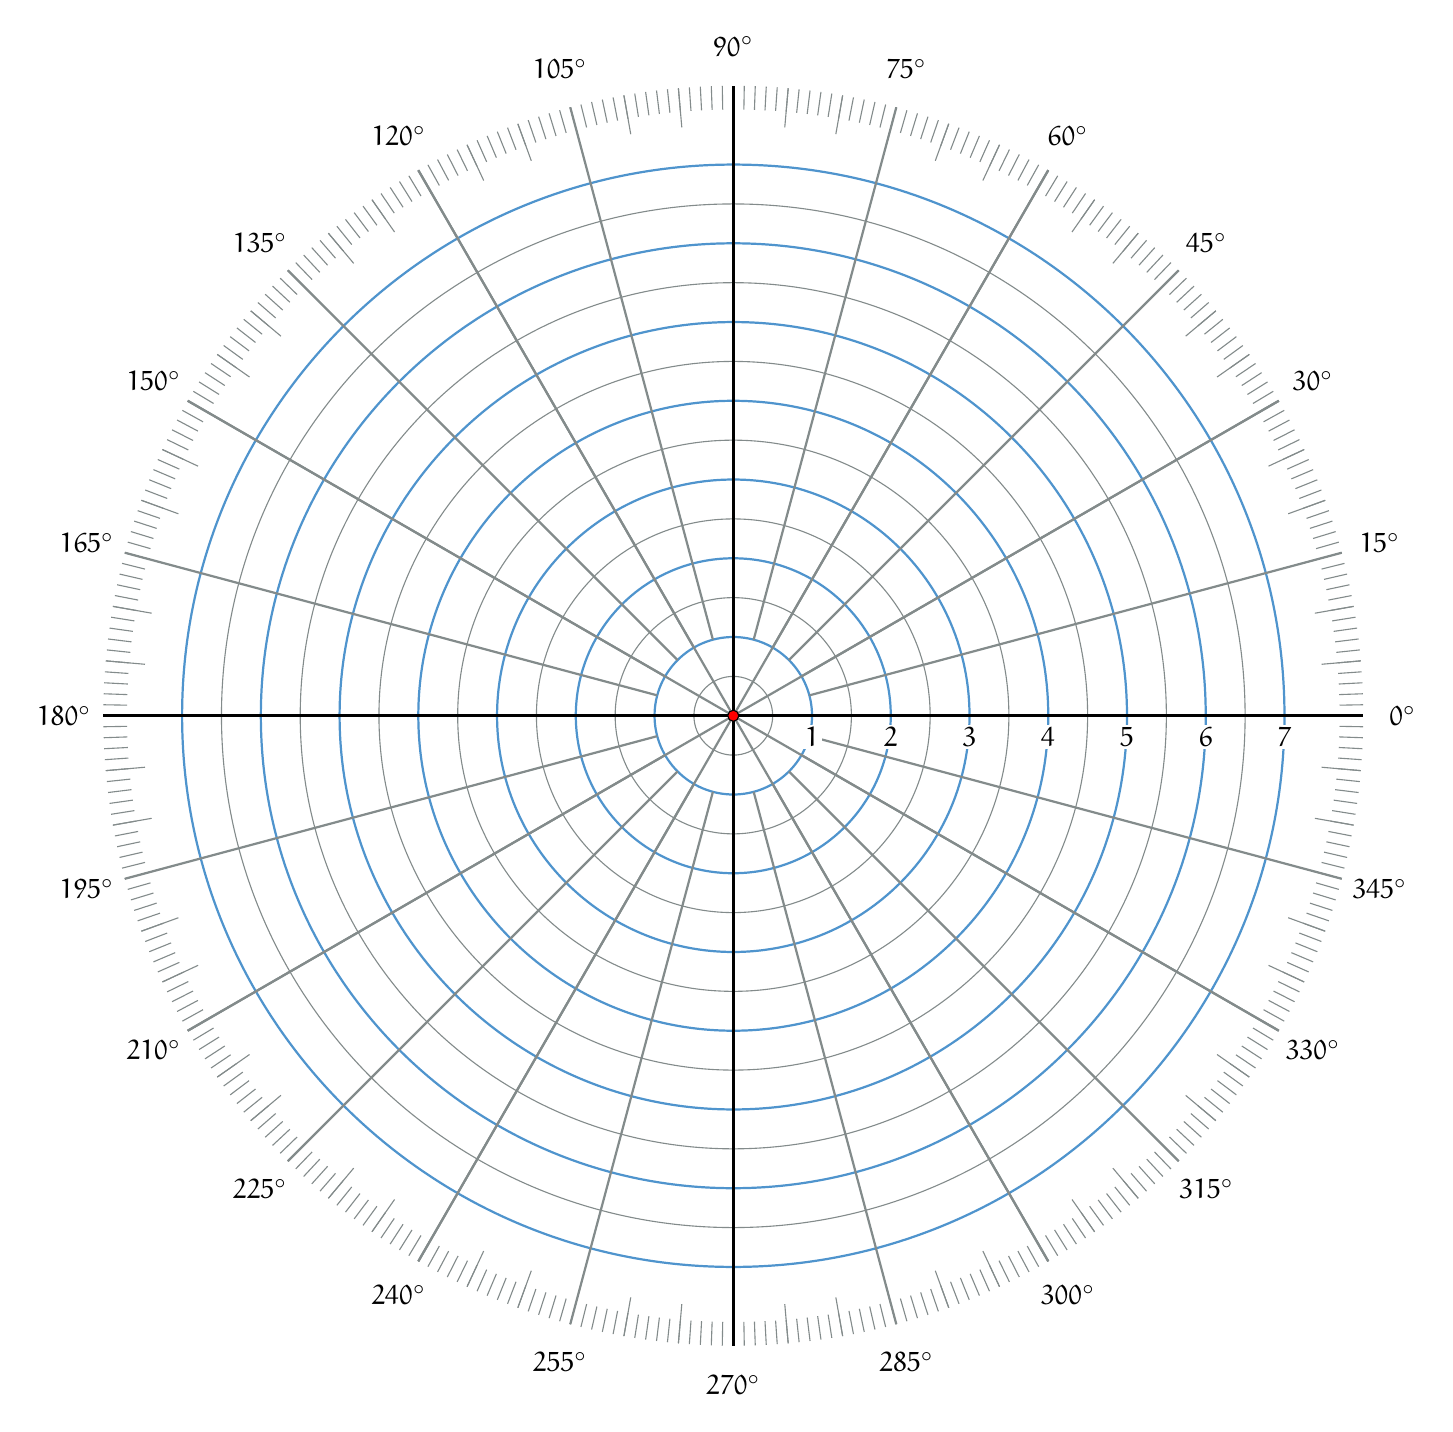
\begin{tikzpicture}
    %Circles 
    \foreach \r in {1, 2,...,7}
      \draw[SteelBlue3, thick] (0,0) circle (\r);    
    \foreach \r in {0.5, 1.5,...,7}
      \draw[Azure4, thin] (0,0) circle (\r);
    %1� Rays
    \foreach \a in {0, 1,...,359}
      \draw[Azure4] (\a:7.7) -- (\a:8);
    %5� Rays
    \foreach \a in {0, 5,...,359}
      \draw[Azure4] (\a:7.5) -- (\a:8);      
    %15� Rays
    \foreach \a in {0, 15,...,359}
      \draw[thick,Azure4] (\a:1) -- (\a:8); 
    %30� Rays
    \foreach \a in {0, 30,...,359}
      \draw[thick,Azure4] (0, 0) -- (\a:8);
    %Radius labels (background filled white)
    \foreach \r in {1, 2,...,7}
      \draw (\r,0) node[inner sep=1pt,below=3pt,rectangle,fill=white] {$\r$};
    %Main rays
    \foreach \a in {0, 90,...,359}
      \draw[very thick] (0, 0) -- (\a:8);
    %Angle labels  
    \foreach \a in {0, 15,...,359}
      \draw (\a: 8.5) node {$\a^\circ$};
    %Central point
    \draw[fill=red] (0,0) circle(0.7mm);
  \end{tikzpicture}
\end{center}

\end{document}
